\everymath{\displaystyle}
\documentclass{beamer}
% \documentclass[handout]{beamer}

%\usepackage[pdftex]{color,graphicx}
\usepackage{amsmath,amssymb,amsfonts}

\mode<presentation>
{
  % \usetheme{Darmstadt}
  % \usetheme[hideothersubsections]{Hannover}
  % \usetheme[hideothersubsections]{Goettingen}
  \usetheme[hideothersubsections, right]{Berkeley}

  \usecolortheme{seahorse}
  % \usecolortheme{dolphin}
  \usecolortheme{rose}
  % \usecolortheme{orchid}

  \useinnertheme[shadow]{rounded}

  \setbeamercovered{transparent}
  % or whatever (possibly just delete it)
}

\mode<handout>{
  \setbeamercolor{background canvas}{bg=black!5}
  \usepackage{pgfpages}
  \pgfpagesuselayout{4 on 1}[a4paper,border shrink=5mm, landscape]
}

\usepackage[brazilian]{babel}
% or whatever

% \usepackage[latin1]{inputenc}
\usepackage[utf8]{inputenc}
% or whatever

\usepackage{times}
% \usepackage[T1]{fontenc}
% Or whatever. Note that the encoding and the font should match. If T1
% does not look nice, try deleting the line with the fontenc.


\title%[Estatística Descritiva I] % (optional, use only with long paper titles)
{Estatística Descritiva I}

\subtitle
{Definições e Distribuições de Frequências} % (optional)

\author%[] % (optional, use only with lots of authors)
{Felipe Figueiredo}% \and S.~Another\inst{2}}
% - Use the \inst{?} command only if the authors have different
%   affiliation.

\institute[INTO] % (optional, but mostly needed)
{
Instituto Nacional de Traumatologia e Ortopedia}
  % \inst{1}%
  % Department of Computer Science\\
  % University of Somewhere
  % \and
  % \inst{2}%
  % Department of Theoretical Philosophy\\
  % University of Elsewhere}
% - Use the \inst command only if there are several affiliations.
% - Keep it simple, no one is interested in your street address.

\date%[Março de 2015] % (optional)
{}

%\subject{Talks}
% This is only inserted into the PDF information catalog. Can be left
% out. 



% If you have a file called "university-logo-filename.xxx", where xxx
% is a graphic format that can be processed by latex or pdflatex,
% resp., then you can add a logo as follows:

\pgfdeclareimage[height=1.6cm]{university-logo}{../logo}
\logo{\pgfuseimage{university-logo}}



% Delete this, if you do not want the table of contents to pop up at
% the beginning of each subsection:
\AtBeginSubsection[]
{
  \begin{frame}<beamer>{Sumário}
    \tableofcontents[currentsection,currentsubsection]
  \end{frame}
}


% If you wish to uncover everything in a step-wise fashion, uncomment
% the following command: 

% \beamerdefaultoverlayspecification{<+->}


\begin{document}

\begin{frame}
  \titlepage
\end{frame}

\begin{frame}{Sumário}
  \tableofcontents
  % You might wish to add the option [pausesections]
\end{frame}


% \section{Análise Descritiva}

% \begin{frame}{Análise Descritiva}
%   \begin{itemize}
%   \item Distribuição de Frequências
%   \item Medidas de Tendência Central
%   \item Medidas de Dispersão
%   \item Medidas de Posição
%   \end{itemize}

% \end{frame}


\section{Tipos de Variáveis}

\begin{frame}{Tipos de Variáveis}
  \begin{definition}
    Variável \alert{dependente} (ou resposta) é a variável a ser
    explicada no estudo.
  \end{definition}
  \begin{definition}
    Variável \alert{independente} (ou explanatória) é a variável que
    serve de suporte na explicação da variabilidade da variável
    resposta.
  \end{definition}
\end{frame}

\begin{frame}{Tipos de Variáveis}
Variáveis podem ser classificadas em duas principais categorias
  \begin{itemize}
  \item Qualitativas (categóricas)
  \item Quantitativas (numéricas)
  \end{itemize}
  \begin{example}
    Pressão sistólica (mmHg), altura (cm), sexo (M ou F), grau de
    satisfação com atendimento médico (nota de 1 a 5), perímetro
    abdominal (cm), contagem de leucócitos, número de pessoas na
    família, cor da pele (branco, negro, pardo), etc.
  \end{example}

\end{frame}

\subsection{Variáveis Qualitativas}

\begin{frame}{Variáveis qualitativas}
Variáveis qualitativas se subdividem em
  \begin{itemize}
  \item<1-2> Nominais
  % \begin{example}
  %   sexo, cor da pele
  % \end{example}

  \item<3-4> Ordinais
  \end{itemize}

  % \begin{example}
  %   satisfação com atendimento médico (nota de 1 a 5)
  % \end{example}

  \begin{example}
    Pressão sistólica (mmHg), altura (cm), \only<2>\alert{sexo (M ou
      F)}, \only<4>\alert{grau de satisfação com atendimento médico
      (nota de 1 a 5)}, perímetro abdominal (cm), contagem de
    leucócitos, número de pessoas na família, \only<2>\alert{cor da
      pele (branco, negro, pardo)}, etc.
  \end{example}

\end{frame}

\subsection{Variáveis Quantitativas}

\begin{frame}{Variáveis quantitativas}
Variáveis quantitativas se subdividem em
  \begin{itemize}
  \item<1-2> Discretos
  \item<3-4> Contínuos
  \end{itemize}
  \begin{example}
    \only<4>\alert{Pressão sistólica (mmHg)}, \only<4>\alert{altura
      (cm)}, sexo (M ou F), grau de satisfação com atendimento médico
    (nota de 1 a 5), perímetro abdominal (cm), \only<2>\alert{contagem
      de leucócitos}, \only<2>\alert{número de pessoas na família},
    cor da pele (branco, negro, pardo), etc.
  \end{example}
\end{frame}

% \section{Tipos de Estudos}
% \begin{frame}{Tipos de Estudos}
%   Estudos podem ser de dois tipos principais
%   \begin{itemize}
%   \item Observacionais
%   \item Experimentais
%   \end{itemize}
% \end{frame}

% \subsection{Estudos experimentais}

% \begin{frame}{Estudos experimentais}
%   \begin{itemize}
%   \item Testar hipóteses em laboratório
%   \item Aleatorização e controle
%   \item Comparam tratamentos (e.g. ensaio clínico)
%   \end{itemize}
%   % \begin{example}
%   %   Ensaios clínicos, testes com animais, etc
%   % \end{example}
% \end{frame}

% \begin{frame}{Estudos experimentais}
%   \begin{example}
%     ``Pesquisadores da Universidade Católica da Coreia testaram com
%     sucesso uma substância do veneno da aranha-armadeira, produzida
%     com células transgênicas de lagarta, para tratar disfunção erétil,
%     em \alert{ratos impotentes}. (...) Para produzir a substância
%     testada, a proteína PnTx2-6, os pesquisadores modificaram células
%     de lagarta com DNA de aranha. Por fim, descobriram que, sob efeito
%     da PnTx2-6, os músculos do corpo cavernoso dos ratos relaxavam,
%     permitindo a entrada de sangue e (eureca!) a ereção.'' Super
%     Interessante, Fevereiro/2015
%   \end{example}
%   \end{frame}

% \subsection{Estudos observacionais}

% \begin{frame}{Estudos observacionais}
%   \begin{itemize}
%   \item Decidir sobre intervenções em populações
%   \item Desenho e controle fogem ao controle do pesquisador
%   % \item Questões éticas
%  \item Comparam populações (e.g. estudos epidemiológicos)
%   \end{itemize}
% \end{frame}

% \begin{frame}{Estudos observacionais}
%   \begin{example}
% %    Prevalência de câncer de esôfago, epidemia de obesidade, etc
%     ``Um grupo de cientistas da Universidade de Harvard descobriu que
%     as bebidas açucaradas industrializadas podem causar 184 mil mortes
%     por ano.  (...) Para chegar ao número, a equipe cruzou os dados
%     correspondentes ao consumo de refrigerantes e sucos no mundo com
%     as mortes por doenças associadas à obesidade. (...) Cerca de 70\%
%     das 184 mil mortes são causadas pela \alert{diabetes}. O resto é
%     por causa de problemas cardíacos e alguns tipos de câncer.'' Super
%     Interessante, Março/2013

%   \end{example}
% \end{frame}

% \begin{frame}{Exercício}
%   O estudo abaixo é experimental ou observacional?
  
%   \begin{block}{Exercício}
%     ``Maconha medicinal não é novidade. A erva já é usada mundo afora
%     com vários objetivos: diminuir dores, náuseas e alguns efeitos
%     secundários de condições como glaucoma, dores nervais e
%     câncer. Agora, em meio a diversos debates sobre a droga,
%     cientistas descobriram que ela pode retardar ou parar
%     completamente a progressão do Mal de Alzheimer. (...)  O estudo
%     revelou que pequenas doses de THC (uma substância química presente
%     na erva) diminuem a concentração de uma proteína chamada
%     beta-amilóide no cérebro. O acúmulo dessa proteína é uma das
%     causas do Alzheimer.'' Super Interessante, Setembro/2014
%   \end{block}
% \end{frame}

\section{Tabelas de Frequências}

\begin{frame}{Frequências de dados}
  \begin{itemize}
  \item Primeiro passo na descrição de grandes datasets: \alert{frequências ou proporções}.
  % \item Quais dados ocorrem com mais frequência?
  % \item Com que proporção eles ocorrem?
  \end{itemize}
  \begin{example}
    \begin{itemize}
    \item Sintomas mais frequentes na amostra de pacientes?
    \item Com que proporção eles ocorrem?
    \end{itemize}
  \end{example}
  \begin{example}
    \begin{itemize}
    \item Qual a proporção de idosos na amostra?
    \end{itemize}
  \end{example}
\end{frame}

\begin{frame}{Tabelas de Frequências de dados}
  \begin{itemize}
  \item Frequência absoluta
  \item Frequência relativa
  \item Frequência acumulada
  \end{itemize}
  \begin{block}{Tipos de dados}
    \begin{itemize}
    \item As frequências absoluta e relativa podem ser determinadas para qualquer tipo de dados
    \item As acumuladas: quantitativos e qualitativos ordinais.
    \end{itemize}
  \end{block}
\end{frame}

\begin{frame}{Tabela de frequências}
  \begin{example}
    Construir uma tabela de distribuições de frequências para o
    seguinte dataset:
    $$ \{ 1,1,1,2,3,3,3,3,3,4,5,5 \}$$
    \begin{center}
      \begin{tabular}[h]{|c|c|c|c|c|}
        \hline
        $x_i$ & $F_i$ & $f_i$ & $F_a$ & $f_a$\\
        \hline
        1 & & & & \\
        \hline
        2 & & & & \\
        \hline
        3 & & & & \\
        \hline
        4 & & & & \\
        \hline
        5 & & & & \\
        \hline
        \hline
        Total & & & & \\
        \hline
      \end{tabular}
      Total de dados: N = 12
    \end{center}
  \end{example}
\end{frame}

\subsection{Frequência absoluta}

\begin{frame}{Frequência absoluta}
  \begin{itemize}
  \item A frequência absoluta ($F$) é a simples contagem da ocorrência
    de cada dado
  \item Soma das frequências: tamanho do dataset.
  \end{itemize}
\end{frame}

\begin{frame}{Tabela de frequências}
  \begin{example}
    Construir uma tabela de distribuições de frequências para o
    seguinte dataset:
    $$ \{ 1,1,1,2,3,3,3,3,3,4,5,5 \}$$
    \begin{center}
      \begin{tabular}[h]{|c|c|c|c|c|}
        \hline
        $x_i$ & $F_i$ & $f_i$ & $F_a$ & $f_a$\\
        \hline
        1 & \alert{\only<2->{3}} & & & \\
        \hline
        2 & \alert{\only<3->{1}} & & & \\
        \hline
        3 & \alert{\only<3->{5}} & & & \\
        \hline
        4 & \alert{\only<3->{1}} & & & \\
        \hline
        5 & \alert{\only<3->{2}} & & & \\
        \hline
        \hline
        Total & \alert{\only<4->{12}} & & & \\
        \hline
      \end{tabular}
      Total de dados: N = 12
    \end{center}
  \end{example}
\end{frame}

\subsection{Frequência relativa}
\begin{frame}{Frequência relativa}
  \begin{itemize}
  \item A frequência relativa ($f$ ou $f\%$) é a frequência absoluta
    dividida pela quantidade total de dados.
  \item Frequências relativas facilitam a comparação de frequências
    entre diferentes datasets.
  \item Soma das frequências: $1 = 100\%$
  \end{itemize}
\end{frame}

\begin{frame}{Tabela de frequências}
  \begin{example}
    Construir uma tabela de distribuições de frequências para o
    seguinte dataset:
    $$ \{ 1,1,1,2,3,3,3,3,3,4,5,5 \}$$
    \begin{center}
      \begin{tabular}[h]{|c|c|c|c|c|}
        \hline
        $x_i$ & $F_i$ & $f_i$ & $F_a$ & $f_a$\\
        \hline
        1 & \only<1>{\alert{3}}\only<2->{3} & \alert{\only<2->{0.25}} & & \\
        \hline
        2 & 1 & \alert{\only<3->{0.08}} & & \\
        \hline
        3 & 5 & \alert{\only<3->{0.42}} & & \\
        \hline
        4 & 1 & \alert{\only<3->{0.08}} & & \\
        \hline
        5 & 2 & \alert{\only<3->{0.17}} & & \\
        \hline
        \hline
        Total & \only<1>{\alert{12}}\only<2->{12} & \alert{\only<3->{1}} & & \\
        \hline
      \end{tabular}
      \only<1-2>{\alert{$\frac{3}{12}=0.25$}}
      \only<3->{Total de dados: N = 12}
    \end{center}
  \end{example}
\end{frame}

\subsection{Frequência acumulada}
\begin{frame}{Frequência acumulada}
  \begin{itemize}
  \item A frequência acumulada mostra a soma gradual das frequências
    de cada dado, em uma tabela ordenada
  \item Absoluta ($F_a$) ou acumulada ($f_a$)
  \end{itemize}
\end{frame}

\begin{frame}{Tabela de frequências}
  \begin{example}
    Construir uma tabela de distribuições de frequências para o
    seguinte dataset:
    $$ \{ 1,1,1,2,3,3,3,3,3,4,5,5 \}$$
    \begin{center}
      \begin{tabular}[h]{|c|c|c|c|c|}
        \hline
        $x_i$ & $F_i$ & $f_i$ & $F_a$ & $f_a$\\
        \hline
        1 & 3 & 0.25 & \alert{\only<1->{3}} & \alert{\only<4>{0.25}}\\
        \hline
        2 & \alert{\only<2>{1}}\only<1,3->{1} & 0.08 & \alert{\only<2->{4}} & \alert{\only<4>{0.33}}\\
        \hline
        3 & 5 & 0.42 & \alert{\only<3->{9}} & \alert{\only<4>{0.75}}\\
        \hline
        4 & 1 & 0.08 & \alert{\only<3->{10}} & \alert{\only<4>{0.83}}\\
        \hline
        5 & 2 & 0.17 & \alert{\only<3->{12}} & \alert{\only<4>{1}}\\
        \hline
        \hline
        Total & 12 & 1 & \alert{\only<3->{12}} & \alert{\only<4>{1}}\\
        \hline
      \end{tabular}
      Total de dados: N = 12
    \end{center}
  \end{example}
\end{frame}

\subsection{Intervalos de Classes}

\begin{frame}{Intervalos de Classes}
  \begin{itemize}
  \item E quanto às variáveis quantitativas contínuas?
  \item Idem discretas quando numerosas?
    \pause
  \item Agrupa-se os dados em classes
  \end{itemize}
  \begin{example}
    A idade (anos) pode ser agrupada em faixas etárias.
  \end{example}
\end{frame}

\begin{frame}{Intervalos de Classes}

  Considere as seguintes alturas (cm):
$ \{ 165,163,170,175,175,174,171,186,159,176,$
$170,158,165,176,169,173,168,172,162,178 \} $

\centering\begin{tabular}{|c|c|c|c|c|}
  \hline
  Altura (cm) & $F$ & $f$ & $F_a$ & $f_a$ \\
  \hline
  $155 |- 160$ & 2 & 0.10 & 2 & 0.10\\%..
  $160 |- 165$ & 2 & 0.10 & 4 & 0.20\\%..
  $165 |- 170$ & 4 & 0.20 & 8 & 0.40\\%....
  $170 |- 175$ & 6 & 0.30 & 14 & 0.70\\%......
  $175 |- 180$ & 5 & 0.25 & 19 & 0.95\\%.....
  $180 |- 185$ & 0 & 0.00 & 19 & 0.95\\%
  $185 |- 190$ & 1 & 0.05 & 20 & 1\\%.
%  $190 |- 195$ & 1 &  &  & \\%
  \hline
  \hline
  Total & 20 & 1 & = & =\\
  \hline
\end{tabular}

\end{frame}
\subsection{Resumo}

\begin{frame}{Frequências x Variáveis}
  \begin{itemize}
  \item Frequências absolutas e relativas
    \begin{itemize}
    \item Todos os tipos de dados
    \end{itemize}
  \item Frequências acumuladas: dados com ordem intrínseca
    \begin{itemize}
    \item Qualitativas Ordinais
    \item Quantitativas Discretas
    \item Quantitativas Contínuas
    \end{itemize}
  \item Classes de dados
    \begin{itemize}
    \item Quantitativas Contínuas
    \item Quantitativas Discretas (se muitos valores possíveis)
    \end{itemize}

  % \item E quanto às variáveis qualitativas nominais?
  \end{itemize}
  
\end{frame}

\section{Gráficos}

\subsection{Visualizando as frequências}

\begin{frame}{Visualizando as frequências}
  \begin{itemize}
  \item Além da tabela, podemos observar \alert{visualmente} as frequências
  \item Diversos tipos de gráficos
  \item Mais comuns: histograma e barras
  \end{itemize}
\end{frame}

\subsection{Histograma}

\begin{frame}{Histograma}
  \begin{itemize}
  \item Construído a partir das frequências de cada \alert{classe} de dados
  \item Cada classe é representada por uma barra (vertical ou horizontal)
  \item Como as classes são contínuas, as \alert{barras} são dispostas \alert{juntas}, na escala
  \end{itemize}
\end{frame}

\begin{frame}{Exemplo}
  \begin{example}
    Alturas (exemplo anterior)

    \bigskip
    \centering $ \{ 165,163,170,175,175,174,171,186,159,176,$
$170,158,165,176,169,173,168,172,162,178 \} $

  \end{example}
\end{frame}

\begin{frame}{Exemplo}
  \begin{center}
    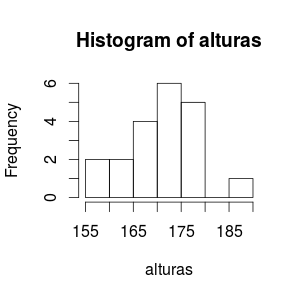
\includegraphics[height=\textheight]{Desc_I/histograma}
  \end{center}
\end{frame}
\begin{frame}{Freqs x Histograma}
  \begin{columns}
    \begin{column}{5cm}
\centering\begin{tabular}{|c|c|}
  \hline
  Altura (cm) & $F$ \\
  \hline
  $155 |- 160$ & 2 \\%..
  $160 |- 165$ & 2 \\%..
  $165 |- 170$ & 4 \\%....
  $170 |- 175$ & 6 \\%......
  $175 |- 180$ & 5 \\%.....
  $180 |- 185$ & 0 \\%
  $185 |- 190$ & 1 \\%.
%  $190 |- 195$ & 1 &  &  & \\%
  \hline
  \hline
  Total & 20 \\
  \hline
\end{tabular}
    \end{column}
    \begin{column}{5cm}
      \begin{center}
        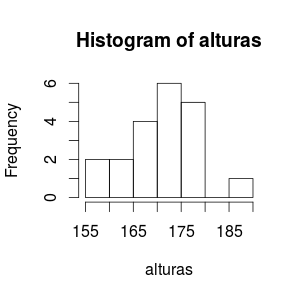
\includegraphics[width=\textwidth]{Desc_I/histograma}
      \end{center}
    \end{column}
  \end{columns}
\end{frame}

\subsection{Barras}

\begin{frame}{Gráfico de barras}
  \begin{itemize}
  \item Frequências de cada ``valor'' que a variável assume
  \item Frequência $\rightarrow$ altura de cada barra
  \item Categorias independentes (semântica)
  \item Histograma x barras: \alert{espaço entre as barras}
  \end{itemize}
\end{frame}

\begin{frame}{Gráfico de barras}
  \begin{example}
    Grau de câncer de uma amostra de pacientes:

    \bigskip
    \centering\{I,\ II,\ I,\ I,\ III\ ,II\ ,I\ ,I\ ,I\}
  \end{example}
  \begin{block}{Pergunta}
    \begin{itemize}
    \item Qual é a classificação dessa variável?
    \end{itemize}
  \end{block}
\end{frame}

\begin{frame}{Frequências}
  \begin{example}
    Grau de câncer de uma amostra de pacientes:

    \bigskip
    \centering\{I,\ II,\ I,\ I,\ III\ ,II\ ,I\ ,I\ ,I\}
  \end{example}
  \begin{block}{Solução}
    \centering\begin{tabular}{|c|c|}
      \hline
      Grau & F\\
      \hline
      \hline
      I & 6\\
      \hline
      II & 2\\
      \hline
      III & 1\\
      \hline
    \end{tabular}
  \end{block}
\end{frame}

\begin{frame}{Gráfico de barras}
  \centering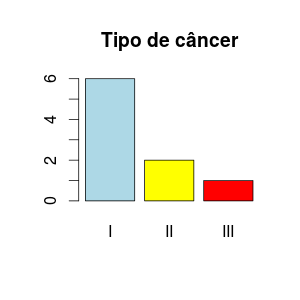
\includegraphics[height=\textheight]{Desc_I/barras}
\end{frame}

\subsection{Pizza}

\begin{frame}{Gráfico de Pizza}
  \begin{itemize}
  \item O gráfico de pizza mostra \alert{exatamente} a mesma informação do gráfico anterior
  \item Frequência $\rightarrow$ área de cada setor
  \item Categorias independentes
  \end{itemize}
\end{frame}

\begin{frame}{Gráfico de Pizza}
  \centering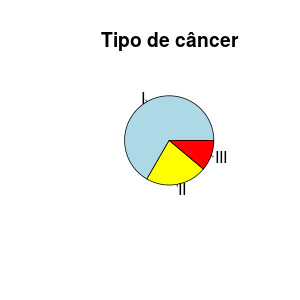
\includegraphics[height=\textheight]{Desc_I/pizza}
\end{frame}

\end{document}

